\documentclass[12pt,a4paper]{article}

% Paquetes básicos
\usepackage[utf8]{inputenc}
\usepackage[T1]{fontenc}
\usepackage[spanish]{babel}
\usepackage{amsmath, amssymb}
\usepackage{siunitx} % Ángulos
\usepackage{graphicx}
\usepackage{float}
\usepackage{geometry}
\usepackage{xcolor}
\geometry{margin=2.5cm}
\usepackage{hyperref}
\usepackage{caption}
\usepackage{subcaption}
\usepackage{setspace}
\usepackage{multirow}
\usepackage{minted}  % Códigos
\usepackage{gensymb} % Grados: "°"
\usepackage[backend=biber, style=ieee]{biblatex}
\usepackage{csquotes}
\usepackage{booktabs}
\addbibresource{Bibliografía.bib}
\graphicspath{{Figuras/}}
\onehalfspacing
\hypersetup{
    colorlinks  = true,
    linkcolor   = blue,    
    citecolor   = blue,
    urlcolor    = blue,
    filecolor   = blue
}


\begin{document}       
\renewcommand{\figureautorefname}{Fig.}
\renewcommand{\tableautorefname}{Tab.}
\renewcommand{\equationautorefname}{Ec.}


% Carátula personalizada
\begin{titlepage}
    \centering
    
\includegraphics[width=0.7\textwidth]{Marvell Logo.png}\\[1.5cm]

    {\Large \textbf{PROGRAMA DE FORMACIÓN MARVELL} \\[0.5cm]}
    {\Large Diseño Digital para Sistemas DSP} \\[0.5cm]

    \rule{\textwidth}{0.5pt} \\[0.5cm]
    {\Large \textbf{Ejercicios Módulo 2: HDL — Sistemas Secuenciales y Combinacionales} \\[0.3cm]}
    \rule{\textwidth}{0.5pt} \\[1cm]
    
\begin{tabular}{l l}
    \textbf{Profesor:} & Del Barco, Martín.\\
    \\[0.5cm]
    \textbf{Alumnos:} & Monja, Ernesto Joaquín\\
                      & Zúñiga, Guillermo Rubén Darío\\
\end{tabular} \\[5cm]

{\centering Año 2026 \par}

\end{titlepage}



% Índice
\tableofcontents
\newpage



\section{Introducción}                                              \label{sec_1}
El presente informe detalla la resolución y simulación de los ejercicios correspondientes al módulo 2 del programa de formación en \textit{Diseño Digital para Sistemas DSP}. A lo largo del documento, se abordan implementaciones en \textit{Verilog} de sistemas secuenciales y combinacionales, evaluando conceptos como el uso correcto de asignaciones, diseño de máquinas de estado finitas (\textit{FSM}) y técnicas de \textit{debugging} en código \textit{RTL}.



\section{Desarrollo}                                                \label{sec_2}
\subsection{Blocking vs Non-Blocking}                               \label{sec_2.1}
En este primer ejercicio se analizó el comportamiento de las asignaciones bloqueantes (\texttt{=}) y no bloqueantes (\texttt{<=}) al intentar implementar un rotador circular con tres registros inicializados en $a = 1$, $b = 2$ y $c = 3$ antes del primer flanco. Se simuló el diseño utilizando \texttt{iverilog} y se observaron los valores en los primeros flancos de reloj.

A partir de la simulación, se obtuvieron los siguientes resultados para ambos casos en los instantes de $10 \, [ns]$ y $20 \, [ns]$, tal como muestra la \autoref{fig:fig_1}.
\begin{figure}[h]
    \centering
    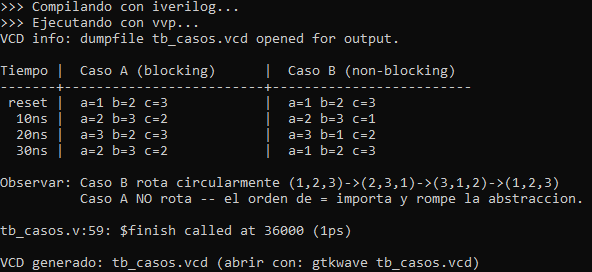
\includegraphics[width=0.8\linewidth]{Figura 1.png}
    \caption{Salida por terminal de la simulación realizada.}
    \label{fig:fig_1}
\end{figure}

Como se puede observar claramente en los resultados, el \textbf{Caso B} es el que implementa un rotador circular real, completando la secuencia $(1,2,3) \rightarrow (2,3,1) \rightarrow (3,1,2) \rightarrow (1,2,3)$. Por el contrario, el \textbf{Caso A} no logra rotar los valores de manera correcta debido a que el orden de las asignaciones bloqueantes importa y rompe la abstracción del hardware. 

En conclusión, el estilo correcto para inferir lógica secuencial (como un registro de desplazamiento o rotador circular) es utilizar asignaciones no bloqueantes (\texttt{<=}) dentro de bloques \texttt{always\_ff}.



\subsection{Registro de 8 Bits con Clock Enable}                    \label{sec_2.2}
Se implementó en Verilog un registro con las siguientes características:
\begin{itemize}
    \item Entrada y salida de 8 bits.
    \item Reset asíncrono, activo por bajo, que establece la salida en 0.
    \item Clock enable síncrono, activo por alto.
\end{itemize}

Luego, se simuló el diseño con un testbench que aplica 10 vectores. Los resultados se muestran a continuación.

\begin{verbatim}
Tiempo  |                     
------- +----------------------------
  100ns | rst=1   ce=1   d=0     q=0
  105ns | rst=1   ce=1   d=2     q=2
  115ns | rst=1   ce=1   d=4     q=4
  125ns | rst=1   ce=1   d=ff    q=ff
  135ns | rst=1   ce=0   d=0     q=ff
  145ns | rst=1   ce=0   d=aa    q=ff
  155ns | rst=1   ce=0   d=1f    q=ff
  160ns | rst=0   ce=0   d=80    q=0
  165ns | rst=0   ce=1   d=40    q=0
  175ns | rst=0   ce=1   d=20    q=0

 - RESULTADOS -
Vector 1: PASS
Vector 2: PASS
Vector 3: PASS
Vector 4: PASS
Vector 5: PASS
Vector 6: PASS
Vector 7: PASS
Vector 8: PASS
Vector 9: PASS
Vector 10: PASS
\end{verbatim}



\subsection{Contador BCD 0-9 con Enable}                             \label{sec_2.3}
Se diseñó un contador decimal \textit{BCD} de $4$ bits que cuenta de $0$ a $9$ y retorna a $0$ (\textit{rollover}). El sistema cuenta con un reset síncrono activo por alto y una señal de habilitación (\texttt{en}). Además, se incluyó una salida (\texttt{tc}) que se activa combinacionalmente durante un único ciclo de reloj cuando el contador alcanza el valor de $9$ y el enable se encuentra activo.

Para la verificación, se elaboró un \textit{testbench} con un reloj de $100 \, [MHz]$ y un bloque \textit{auto-checker} integrado. Se ejecutó una simulación de $100$ ciclos de reloj continuos con la señal de enable activa, tras los cuales el sistema reportó por consola el estado \textbf{[ PASS ]}, contabilizando exitosamente 10 pulsos exactos de la señal \texttt{tc} tal como muestra la \autoref{fig:fig_2}.
\begin{figure}[H]
    \centering
    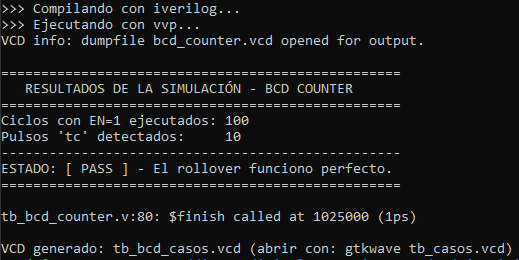
\includegraphics[width=0.8\linewidth]{Figura 2.png}
    \caption{Salida por terminal de la simulación realizada.}
    \label{fig:fig_2}
\end{figure}

Finalmente, se generó un archivo \textit{VCD} para inspeccionar visualmente las señales mediante la herramienta \textit{GTKWave}. En la \autoref{fig:fig_3} se aprecian las formas de onda resultantes de la simulación.
\begin{figure}[H]
    \centering
    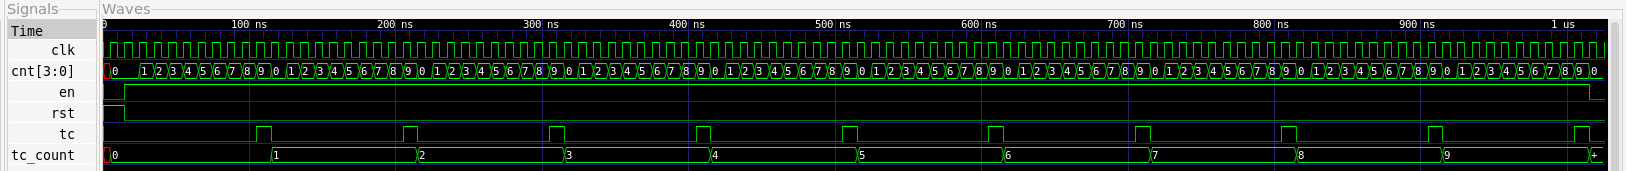
\includegraphics[width=1\linewidth]{Figura 3.png}
    \caption{Formas de onda de la simulación del contador \textit{BCD} en \textit{GTKWave}.}
    \label{fig:fig_3}
\end{figure}

A través del diagrama temporal se constata el comportamiento esperado del \textit{HW}. Se observa la correcta inicialización mediante el reset síncrono en el primer flanco de reloj, el ciclo de \textit{rollover} que salta de $9$ a $0$ sin estados intermedios, y la generación instantánea del pulso \texttt{tc} sin desfasajes de reloj. Esto último valida la implementación exitosa de la separación entre la lógica secuencial (el contador) y la lógica combinacional (la bandera de fin de cuenta).



\subsection{FSM Detector de Secuencia ``101''}                      \label{sec_2.4}
Se implementó una \emph{máquina de estados finita} (FSM) que levanta una salida cuando detecta la secuencia ``101'' en una entrada serial. Por ejemplo, si la entrada es de secuencia \texttt{110101} la salida tiene la secuencia \texttt{000101}.

El detector se comporta según el diagrama de estados de la \autoref{fig:fig_4} y tiene las siguientes características:
\begin{itemize}
    \item 1 bit de entrada y de salida.
    \item Reset asíncrono activo por bajo.
    \item Codificación binaria.
    \item Sigue el modelo de Moore.
\end{itemize}

\begin{figure}[H]
    \centering
    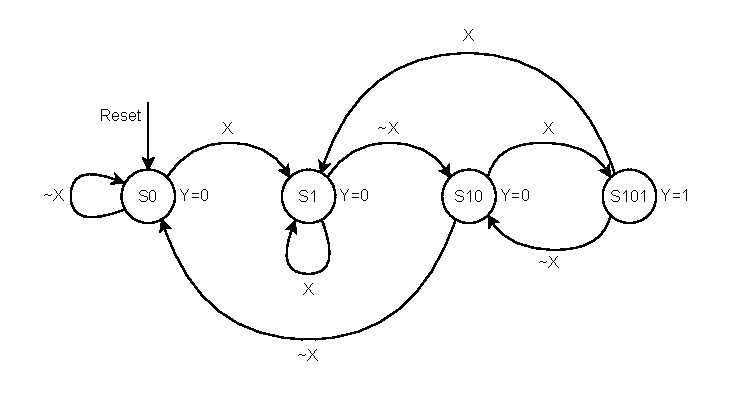
\includegraphics[width=0.7\linewidth]{Figura 4.pdf}
    \caption{Diagrama de estados de la FSM.}
    \label{fig:fig_4}
\end{figure}

En el testbench se produjo la salida a continuación:

\begin{verbatim}
Tiempo  |                                                   
------- +-------------------------------------------------------
  115ns | x = 0          y(esperado) = 0         y(obtenido) = 0
  125ns | x = 1          y(esperado) = 0         y(obtenido) = 0
  135ns | x = 1          y(esperado) = 0         y(obtenido) = 0
  145ns | x = 0          y(esperado) = 0         y(obtenido) = 0
  155ns | x = 1          y(esperado) = 1         y(obtenido) = 1
  165ns | x = 0          y(esperado) = 0         y(obtenido) = 0
  175ns | x = 1          y(esperado) = 1         y(obtenido) = 1
  185ns | x = 1          y(esperado) = 0         y(obtenido) = 0
  195ns | x = 0          y(esperado) = 0         y(obtenido) = 0
  205ns | x = 1          y(esperado) = 1         y(obtenido) = 1
  215ns | x = 0          y(esperado) = 0         y(obtenido) = 0
  225ns | x = 1          y(esperado) = 1         y(obtenido) = 1
  235ns | x = 0          y(esperado) = 0         y(obtenido) = 0
  245ns | x = 0          y(esperado) = 0         y(obtenido) = 0
  255ns | x = 1          y(esperado) = 0         y(obtenido) = 0
  265ns | x = 0          y(esperado) = 0         y(obtenido) = 0
  275ns | x = 1          y(esperado) = 1         y(obtenido) = 1
\end{verbatim}




\subsection{Pipeline 3-etapas con Valid/Ready}                      \label{sec_2.5}
En este ejercicio se diseñó un \textit{pipeline} de $3$ etapas encargado de calcular la expresión aritmética presentada en la \autoref{eq_1}, procesando muestras de $8$ bits con signo (\texttt{signed}) y utilizando las constantes fijadas por consigna $A = 5$ y $B = 3$. 
\begin{equation}
    y = ((x + A) \ast B) \gg 4
    \label{eq_1}
\end{equation}

La interfaz del módulo se construyó respetando el protocolo de \textit{handshake AXI-Stream} mientras que para implementar la lógica de \textit{back-pressure}, se utilizó la señal de entrada \texttt{ready\_in} como un \textit{Clock Enable} común para todos los \textit{Flip-Flops} del diseño. De esta forma, cuando el receptor no está listo (\texttt{ready\_in} $= 0$), el sistema entra en estado de \textit{stall}, congelando el procesamiento y propagando la condición hacia la entrada mediante \texttt{ready\_out}.

La validación funcional se realizó mediante un \textit{testbench} equipado con un \textit{golden model} por software y una estructura de datos tipo \textit{FIFO} para gestionar la latencia temporal de las muestras. Se evaluaron $2$ escenarios:
\begin{itemize}
    \item \underline{Fase 1 (Régimen ideal):} Transmisión continua sin \textit{stalls}. El \textit{throughput} observado se alineó con el rendimiento teórico de $1$ muestra/ciclo (procesando $20$ muestras en $26$ ciclos, contemplando latencias de llenado y vaciado).
    \item \underline{Fase 2 (Régimen con \textit{stalls}):} Se introdujeron cortes aleatorios en la señal \texttt{ready\_in}, verificando que no existiera pérdida ni sobreescritura de datos.
\end{itemize}
\begin{figure}[H]
    \centering
    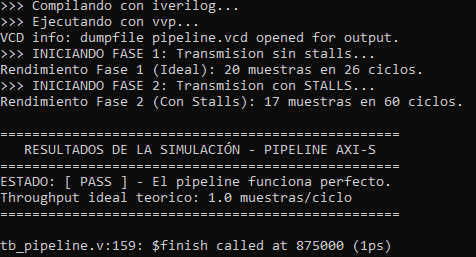
\includegraphics[width=0.7\linewidth]{Figura 5.png}
    \caption{Salida por terminal de la simulación realizada.}
    \label{fig:fig_5}
\end{figure}

El verificador automático reportó cero errores. En la \autoref{fig:fig_6} se aprecian las formas de onda capturadas durante la simulación.
\begin{figure}[H]
    \centering
    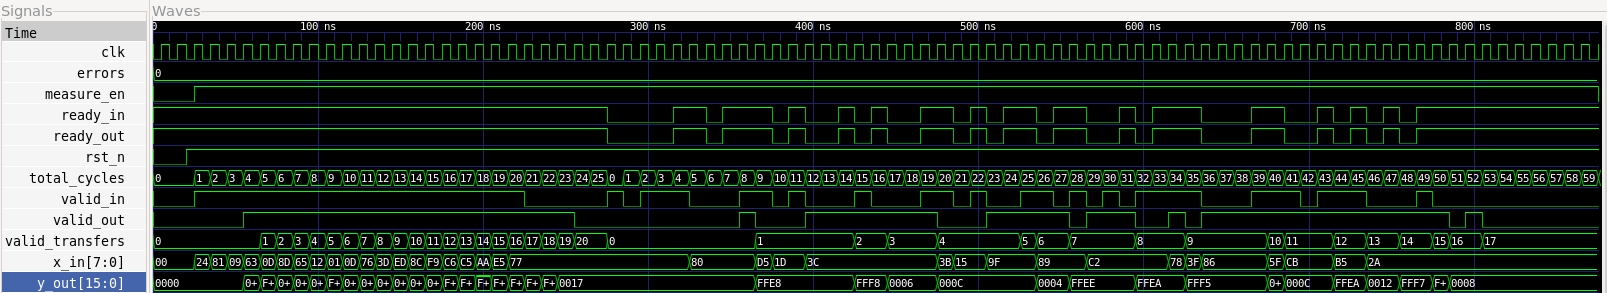
\includegraphics[width=1\linewidth]{Figura 6.png}
    \caption{Simulación del pipeline evidenciando la latencia de $3$ ciclos y el comportamiento ante \textit{stalls}.}
    \label{fig:fig_6}
\end{figure}

A partir del análisis temporal, se confirma el correcto comportamiento del flujo de datos. Se aprecia claramente el desfasaje inicial de 3 ciclos hasta la activación de \texttt{valid\_out}, y cómo las señales y datos internos se mantienen estables cada vez que \texttt{ready\_in} cae a nivel bajo, comprobando la robustez de la lógica de \textit{back-pressure}.



\subsection{Debugging de Latch Oculto}                              \label{sec_2.6}




\section{Conclusiones}                                              \label{sec_3}
[Completar]



\newpage
\printbibliography[heading=bibintoc, title={4. \ Referencias}]
\end{document}